\begin{figure*}[ht]
	\renewcommand\arraystretch{0.4}
	\begin{tabular}{@{}p{1.5cm}@{}c@{}c@{}c@{}c@{}c@{}c@{}c}
	\raisebox{10mm}{\small RGB} &  
	
\includegraphics[width=0.130\linewidth]{fig/qual/rgb/image_0303.png} & 
	
\includegraphics[width=0.130\linewidth]{fig/qual/rgb/image_0520.png} &
	\includegraphics[width=0.130\linewidth]{fig/qual/rgb/image_0825.png} & 
	\includegraphics[width=0.130\linewidth]{fig/qual/rgb/image_0946.png} & 
	
\includegraphics[width=0.130\linewidth]{fig/qual/rgb/image_0996.png} & 
	\includegraphics[width=0.130\linewidth]{fig/qual/rgb/image_0198.png} & 
	\includegraphics[width=0.130\linewidth]{fig/qual/rgb/image_0440.png} \\
	\raisebox{10mm}{\small Depth} &  
	
\includegraphics[width=0.130\linewidth]{fig/qual/depth/image_0303.png} &  
	
\includegraphics[width=0.130\linewidth]{fig/qual/depth/image_0520.png} &
	\includegraphics[width=0.130\linewidth]{fig/qual/depth/image_0825.png} &
	\includegraphics[width=0.130\linewidth]{fig/qual/depth/image_0946.png} &
	
\includegraphics[width=0.130\linewidth]{fig/qual/depth/image_0996.png} &
	\includegraphics[width=0.130\linewidth]{fig/qual/depth/image_0198.png} &
	\includegraphics[width=0.130\linewidth]{fig/qual/depth/image_0440.png} \\
	\raisebox{10mm}{\small FORTH} &  
	
\includegraphics[width=0.130\linewidth]{fig/qual/forth/image_0303.png} & 
	
\includegraphics[width=0.130\linewidth]{fig/qual/forth/image_0520.png} &
	\includegraphics[width=0.130\linewidth]{fig/qual/forth/image_0825.png} &
	\includegraphics[width=0.130\linewidth]{fig/qual/forth/image_0946.png} &
	
\includegraphics[width=0.130\linewidth]{fig/qual/forth/image_0996.png} &
	\includegraphics[width=0.130\linewidth]{fig/qual/forth/image_0198.png} &
	\includegraphics[width=0.130\linewidth]{fig/qual/forth/image_0440.png} \\
	\raisebox{10mm}{\parbox{1.3cm}{\small Classfication\\(Ours)}} &  
	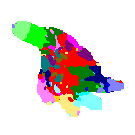
\includegraphics[width=0.130\linewidth]{fig/qual/class/class-303.png} & 
	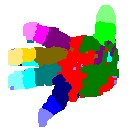
\includegraphics[width=0.130\linewidth]{fig/qual/class/class-520.png} &
	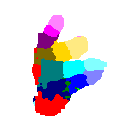
\includegraphics[width=0.130\linewidth]{fig/qual/class/class-825.png} & 
	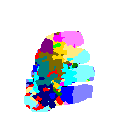
\includegraphics[width=0.130\linewidth]{fig/qual/class/class-946.png} &
	
\includegraphics[width=0.130\linewidth]{fig/qual/class/class-996.png} &
	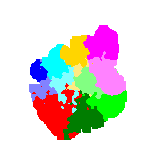
\includegraphics[width=0.130\linewidth]{fig/qual/class/class-198.png} &
	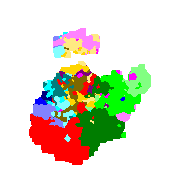
\includegraphics[width=0.130\linewidth]{fig/qual/class/class-440.png} \\
	\raisebox{10mm}{\small Regression} &  
	
\includegraphics[width=0.130\linewidth]{fig/qual/vote/image_0303.png} & 
	
\includegraphics[width=0.130\linewidth]{fig/qual/vote/image_0520.png} & 
	\includegraphics[width=0.130\linewidth]{fig/qual/vote/image_0825.png} & 
	\includegraphics[width=0.130\linewidth]{fig/qual/vote/image_0946.png} &
	
\includegraphics[width=0.130\linewidth]{fig/qual/vote/image_0996.png} &
	\includegraphics[width=0.130\linewidth]{fig/qual/vote/image_0198.png} &
	\includegraphics[width=0.130\linewidth]{fig/qual/vote/image_0440.png} \\
	& 
	{\small (a) Sequence $B$} &
	{\small (b) Sequence $B$} & 
	{\small (c) Sequence $B$} & 
	{\small (d) Sequence $B$} & 
	{\small (e) Sequence $B$} & 
	{\small (f) Sequence $C$} & 
	{\small (g) Sequence $C$} \\ 
	& {\small \ \ \ Frame 303} &
	{\small \ \ \ Frame 520} & 
	{\small \ \ \ Frame 825} & 
	{\small \ \ \ Frame 946} & 
	{\small \ \ \ Frame 996} & 
	{\small \ \ \ Frame 99} & 
	{\small \ \ \ Frame 223} \\ 
	\end{tabular}
\caption{Qualitative results of the multi-view experiment. Hand regions are cropped from the original images for better visualisation ($135\times135$ pixels for sequence $B$, $165\times165$ pixels for sequence $C$); the size of the origin images (RGB and depth) is $640\times480$ pixels. Colour scheme of joint labels refer to Figure~\ref{fig:experiments:singleview}.}
	\label{fig:experiments:multiview:qual}
\end{figure*}
